\documentclass{article}

\title{Estatística Numérica Computacional\\Trabalho nº1}
\author{Marta Paz nº49861\\
		Rafael Almeida nº49788\\
		Rafael Gameiro nº50677\\
		Ricardo Pinto nº49811\\
}
\date{October, 2018}

\usepackage{amsmath}
\usepackage{graphicx}

\begin{document}
	\maketitle
	\pagenumbering{gobble}
	\newpage
	\pagenumbering{arabic}
	
	
	\section*{Exercício 1}
		\paragraph{}
			Considere a variável aleatória X com função densidade de probabilidade
			\begin{equation*}
				f(x) = \begin{cases} 
						3x^2, & 0 < x < 1 \\\\ 0, & \mbox{para outros valores de x} 
					\end{cases}
			\end{equation*}
	
			Considere agora a variável aleatória $Y = g(X)$, sendo $g(x) = log(2x^2 + 3)$. Estime $P(1 < Y < 1.5)$ usando o método de Monte Carlo e apresente também o desvio padrão da estimativa.
	
		\subsection*{Resolução}
			\paragraph{}
				1. Sabendo que $0 < x < 1$, pelo ramo da função onde x varia, e que g é crescente (isto porque a função logarítmica cresce ao tender para mais infinito), então podemos concluir que $g(0) < g(X) < g(1)$.
De outro modo, substituindo as expressões pelos seus valores respetivos, temos: $1,099 < Y < 1,61$.\\
				Assim:
				
					\begin{align*}	
				 P(1 < Y < 1.5) &= P(1 < Y < 1.099) + P(1.099 < Y < 1.61)\\ 
				 &= 0 + P(1.099 < Y < 1.61) = P(g^{-1}(1.099) < X < g^{-1}(1.61))
				 	\end{align*}

				2. De seguida, calculámos o valor de $g^{-1}(x)$:
					\begin{equation*}
						\begin{aligned}
							y = log(2x^2 + 3) &\Leftrightarrow e^y = 2x^2 + 3
							\Leftrightarrow x^2 = \frac{e^y - 3}{2}\\ 
							&\Leftrightarrow x = \sqrt{\frac{e^y - 3}{2}}
							\Leftrightarrow g^{-1}(x) = \sqrt{\frac{e^y - 3}{2}}
						\end{aligned}
					\end{equation*}		
				\indent 3. Ficamos, assim, com o integral,
					\begin{equation*}
						\int^{g^{-1}(1.61)}_{g^{-1}(1.099)} f(x) dx
					\end{equation*}							
					onde aplicámos o método de Monte Carlo em R.
\newpage				
			\begin{figure}[!h]
				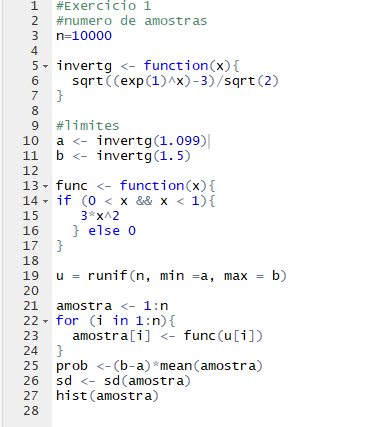
\includegraphics[scale=0.40]{ex1}
			\end{figure}	
				\indent R: $P(1< Y < 1.5) \approx 0.64 $ \indent sd$ \approx 0.66$	
		

		
	\section*{Exercício 2}
			\noindent Sejam X e Y duas variáveis aleatórias independentes ambas com função densidade de probabilidade, $f(x) = \frac{2}{\sqrt{2\pi}}.e^{-\frac{x^2}{2}}$, $0 < x < +\infty $, (ou seja, estas variáveis são o valor absoluto de uma normal standart) e seja $\theta = E(e^{X + Y})$.
			
			\paragraph{}
			\textbf{a)} Use o método de Monte Carlo para estimar $\theta$, usando variáveis aleatórias com distribuição $Unif(0, 1)$.
				
				\subsubsection*{Resolução}
				\paragraph{}
					Para este exercício, efetuámos uma mudança de variável para que o integral que queremos calcular que é:
					
					\begin{equation*}
						\int^{+\infty}_{0}\int^{+\infty}_{0} e^{x + y} dxdy
					\end{equation*}
					
					\noindent Para que o domínio de integração esteja entre 0 e 1, fizemos a seguinte conta:
					
					\begin{equation*}
						u = \frac{1}{x + 1} \Leftrightarrow 
						{(x + 1)u = 1} \Leftrightarrow 
						(x + 1) = \frac{1}{u} \Leftrightarrow 
						{x = \frac{1}{u} - 1} \Leftrightarrow 
						x = \frac{1-u}{u}
					\end{equation*}
					\begin{equation*}
						\begin{aligned}
							u(0) = \frac{1}{0 + 1} = 1 = b\\
							u(+\infty) = \frac{1}{+\infty + 1} = 0 = a
						\end{aligned}
					\end{equation*}
					\textbf{Nota}: a mudança de variável para o y é igual à de x, mas como x e y são variáveis independentes tem-se de usar uma letra diferente
					\begin{equation*}
						\int^{1}_{0}\int^{1}_{0} e^{\left(\frac{2}{\sqrt{2\pi}}.e^{-\frac{\left(\frac{(1-u)}{u}\right)^2}{2}}\right)}.
						e^{\left(\frac{2}{\sqrt{2\pi}}.e^{-\frac{\left(\frac{(1-t)}{t}\right)^2}{2}}\right)}.{-\frac{1}{u^2}}.{-\frac{1}{t^2}}dudt
					\end{equation*}					
					
			\noindent Como não conseguimos calcular este integral analiticamente vamos recorrer ao método de Monte Carlo para calcular uma estimativa para o seu valor.\\
				       Para tal, fizemos os seguintes passos em R:\\					
			\indent 1. Criámos uma função auxiliar que nos vai dar a fórmula da expressão que queremos calcular o estimador, e consequentemente, o integral\\
			\indent 2. Criámos uma amostra aleatória para o valor de x e outra para o valor de y\\
			\indent 3. Em seguida, calculámos o valor da expressão com os valores aleatórios e obtivemos o resultado do estimado, calculando a média de todos os valores 
			
					\begin{figure}[!h]
						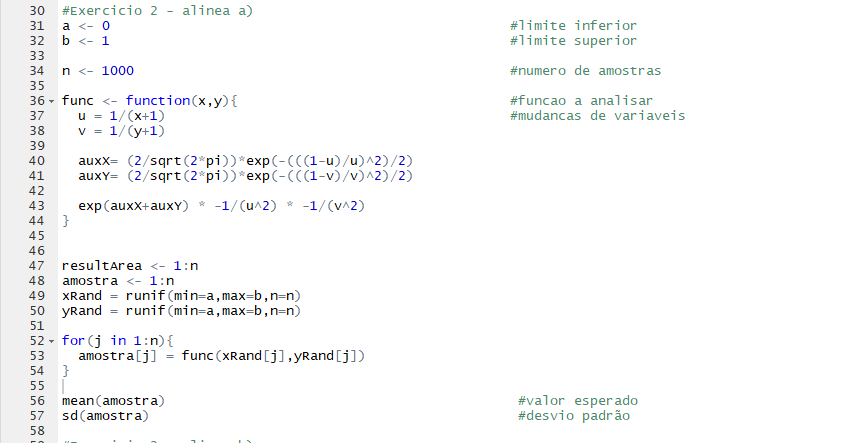
\includegraphics[scale=0.5]{ex2a)}
					\end{figure}		
					\indent R: $\approx 20.16$

\newpage

			\paragraph{}
			\textbf{b)} Reestime o parâmetro $\theta$ através do método de Monte Carlo usando agora variáveis aleatórias com outra distribuição, uma distribuição que considere adequada.

				\subsubsection*{Resolução}
				\paragraph{}
					\indent 1. Para este exercício, considerámos que a distribuição mais adequada para calcular as variáveis aleatórias seria utilizar a distribuição normal, uma vez que duas vezes a função densidade de probabilidade da normal é igual à função densidade de probabilidade das variáveis X e Y.
				\paragraph{}
					\indent 2. Assim sendo, no R, geramos 1000 valores aleatórios com distribuição uniforme para duas variáveis diferentes e de seguida aplicámos a tranformação de Box-Muller para obtermos distribuições normais. Depois, para cada valor gerado nas duas variáveis anteriores, calculámos $exp(Xi+Yi)$.
				\paragraph{}
					\begin{figure}[!h]
						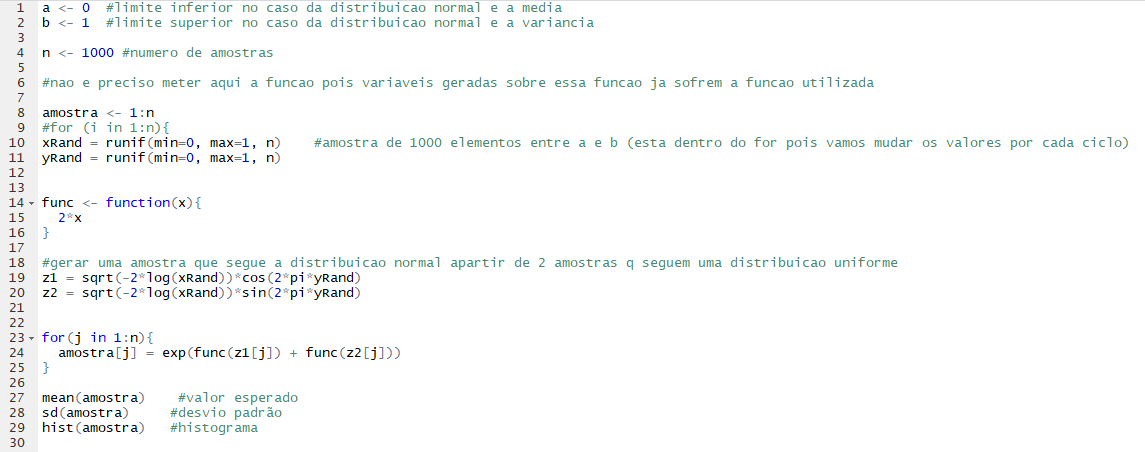
\includegraphics[scale=0.75]{ex2b)}
					\end{figure}		
					\indent R: $\theta \approx 35.6$

			\paragraph{}
			\textbf{c)} Considere o estimador de Monte Carlo da alínea (a), $\hat{\theta}$ e seja $C=\overline{UV}$, ou seja, $C=\frac{1}{N}\sum\limits_{i=1}^n{U_{i}V_{i}}$ uma variável de controlo, em que $U$ e $V$ são variáveis aleatórias com distribuição Unif(0,1). Reestime $\theta$ usando esta variável de controle. Estime o desvio-padrão e compare os desvios-padrão dos dois estimadores. Discuta os resultados numéricos e analíticos. 
	
				\subsubsection*{Resolução}
				\paragraph{}
					\indent 1. Para resolver este exercício, utilizámos a seguinte fórmula para reestimar a variável 
				\paragraph{}
					\begin{equation*}
					     \hat{\theta}c =  \hat{\theta} - \beta*(C - E(u))
					\end{equation*}
				\paragraph{}
					\indent 2. Para tal, utilizámos parte do código feito no exercicio (a) e gerámos uma variável de controle apartir da função generateControl implementada no R.
				\paragraph{}
					\indent 3. De seguida, tivemos de calcular um  $\beta$. Para calcular este valor, usámos a seguinte fórmula:
				\paragraph{}
					\begin{equation*}
						\beta=\frac{(Cov(\hat{\theta},C))}{Var(c)}
					\end{equation*}
				\paragraph{}
						Para calcular o beta, criámos uma função no R, que calcula a covariância entre a variavel de controle dada e a amostra calculada do exercicio a). Para além do cálculo da covariância, também tivemos de calcular a variância da variável de controle, C.
				\paragraph{}
					\indent 4. De seguida, gerámos uma nova amostra seguindo a seguinte formula:
				\paragraph{}
					\begin{equation*}
						finalC[i] = amostra[i] - (\beta*(c[i] - mean(c)))
					\end{equation*}
				\paragraph{}
				\paragraph{}
					\indent 5. A média dessa amostra é o estimador que queremos calcular que terá o seguinte valor:  $\hat{\theta}c = 19.98$ 
				\paragraph{}
					\indent 6. O valor do desvio padrão de  $\hat{\theta}c = 8.014776$ e o valor do desvio padrão de $\hat{\theta} = 8.017608$, sendo que obtivemos o mesmo valor para o valor do estimador.
				\paragraph{}
					\indent 7. Comparando os valores apresentados no ponto 6, podemos verificar que, usando a variável de controlo, o valor do estimador fica igual ao valor do estimador quando não utilizávamos a variável de controlo, mas, em contrapartida, o valor do desvio padrão desce ligeiramente quando o estimador é calculado com a variável de controlo. Assim, podemos concluir que o cálculo de um estimador é mais preciso e/ou as variáveis aleatórias geradas estão mais próximas do valor real.

				\newpage
				\begin{figure}[!h]
						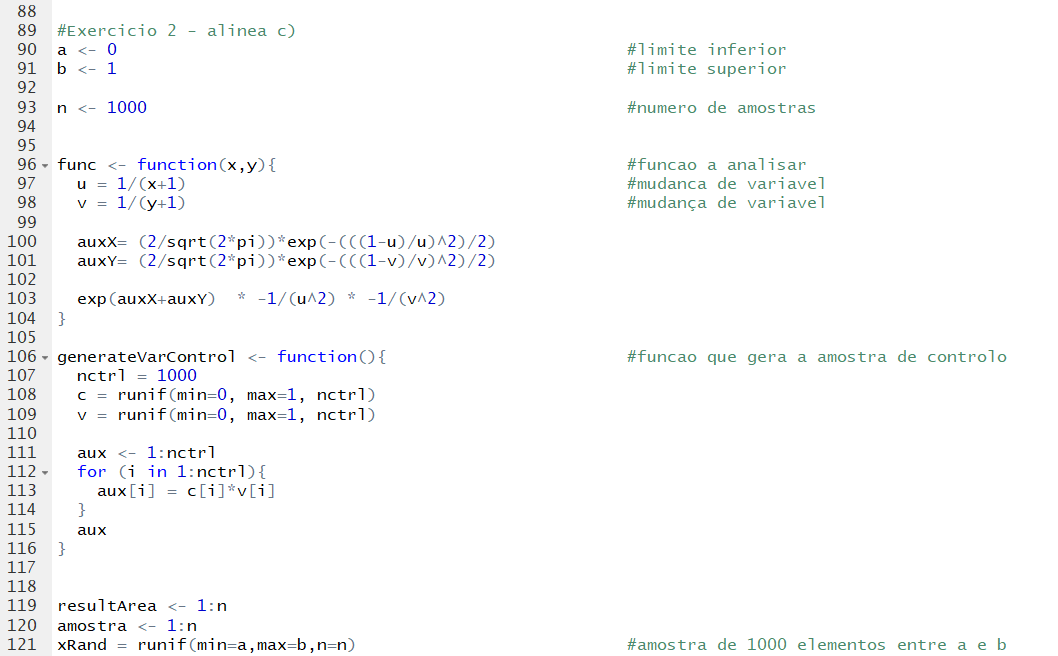
\includegraphics[scale=0.6]{ex2c)}
				\end{figure}	
				\begin{figure}[!h]
						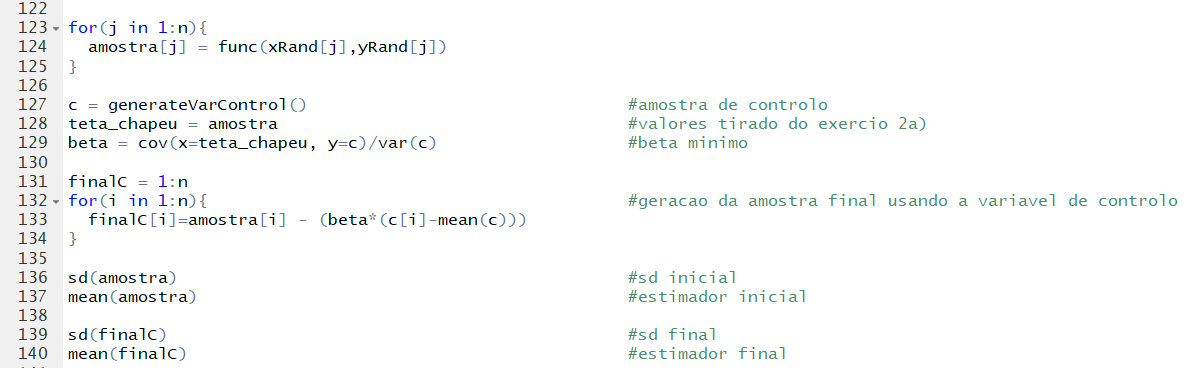
\includegraphics[scale=0.6]{ex2c)cont}
				\end{figure}	
	
\end{document}
